% Preamble
\documentclass[11pt, twoside]{report}

% Packages

\usepackage[utf8]{inputenc}
\usepackage[T1]{fontenc}                            %Sets fontenc to max level needed in file
\usepackage{graphicx}                               %To load and display images
\usepackage{caption}                                %For subfigures and cap env
\usepackage{subcaption}
\usepackage[a4paper, width=150mm,                   %Size of Paper
            top=25mm, bottom=25mm,
            bindingoffset=6mm]{geometry}
\usepackage{fancyhdr}                               %Header and Footers
\pagestyle{fancy}                                   %To disable for specific page use \pagestyle{<type>}
                                                    %<type>: plain for pagenr
                                                        %    empty for empty pagestyle
                                                        %    fancy to enable the default syle again
\fancyhead{}                                        %Resets the header
\fancyhead[RO,LE]{\chaptername~\thechapter}         %Header Definition: Chaptername and number: Right on Odd and Left on even pages
\fancyfoot{}                                        %Resets the footer
\fancyfoot[CE, CO]{\thepage}                        %Centered Page Number on odd and even pages
%Define output dir, because of error with: https://tex.stackexchange.com/questions/112953/error-when-using-minted-package-and-output-directory-option
%Cache can be removed normally, but in certain situations it can result in errors. Setup minted see: https://alipourmousavi.com/blog/index.php/2018/02/08/using-minted-package-in-latex-to-format-codes/
\usepackage[cache=false, outputdir=Z:/Users/jan22/CodeProjects/latex_template/auxil]{minted} %Must be before csquotes
\setminted{
    linenos=true,
    autogobble
}
\usepackage[english]{babel}                         %For splitting words
\usepackage{csquotes}                               %Used for babel/polyglossia and minted
\usepackage{setspace}                               %Set line spaceing
\setstretch{1.5}
\usepackage{amsmath}                                %Math package
\usepackage{color}                                  %Colored Links
\usepackage{hyperref}                               %For setting links
\hypersetup{
    colorlinks=false,                                %true, if links should be colorful
    linktoc=all,                                    %all => sections and subsections linked
    linkcolor=black,                                %Color of link
}
\usepackage{listings}                               %Environment for listings
%\usepackage{eurosym}                               %Euro sign
%Maybe change back to biber
\usepackage[style=authoryear,citestyle=authoryear,backend=bibtex]{biblatex}   % Bib
\addbibresource{main.bib}                           %Set bib file

%FOR minted
\renewcommand{\MintedPygmentize}{Z:/Users/jan22/AppData/Local/Programs/Python/Python37-32/Scripts/pygmentize} %Set path to script location
\renewcommand{\theFancyVerbLine}{\sffamily\textcolor[rgb]{0.5,0.5,0.5}{\scriptsize\arabic{FancyVerbLine}}}
% Create a new environment for breaking code listings across pages.
%Change lstlisting to figure if code fragments should be listed under figures
\newenvironment{longlisting}{\captionsetup{type=lstlisting}}{}
\renewcommand{\lstlistingname}{Code Fragment}       %Sets name of Listing space lstlisting - Will occured before each caption inside its environment
\renewcommand{\lstlistlistingname}{List of \lstlistingname s} %Sets title for \listoflstlistings




%CUSTOM VARS:
\newcommand{\submissionDay}{day-of-submission}
\newcommand{\submissionMonth}{month-of-submission}
\newcommand{\submissionYear}{year-of-submission}
\newcommand{\maintitle}{thesis-title}
\newcommand{\subtile}{thesis-title-addition}
\newcommand{\name}{author-title-name}
\newcommand{\supervisor}{supervisor-title-name}

% Document
\begin{document}
    % Titelblatt:
% \newpage\mbox{}\newpage
\cleardoublepage   % force output to a right page
\thispagestyle{empty}
\begin{titlepage}
    \begin{flushright}
        
\includegraphics[width=0.4\linewidth]{../src/other-pages/title/Logo-A3.jpg}
    \end{flushright}
    %! Suppress = LineBreak
    \begin{flushleft}
        \vspace{0.5cm}

        \section*{\maintitle}
        %\subsection*{\subtile}

        \vspace{0.5cm}

        Bachelor Thesis 2\\
        In Partial Fulfillment
        of the Requirements for the Degree of
        Bachelor of Science

        \vspace{0.5cm}

        \textbf{Bachelor of Science in Software and Information Engineering}

        \vspace{1cm}
        University of Applied Sciences FH Vorarlberg\newline
        Software and Information Engineering

        \vspace{0.5cm}

        Supervised by:\newline
        \phantom{x}\hspace{3ex}\supervisor\newline
        \vspace{0.5cm}

        Submitted by:\newline
        \phantom{x}\hspace{3ex}\name\newline
        \newline
        Dornbirn, \submissionMonth\space\submissionYear
    \end{flushleft}
\end{titlepage}

\newpage
\addtocontents{toc}{\protect\setcounter{tocdepth}{-1}}
\chapter*{Abstract}\label{ch:abstract}
Text

\chapter*{AbstractGER}\label{ch:abstractger}
Text

\addtocontents{toc}{\protect\setcounter{tocdepth}{2}}
\newpage
%Table of contents
\tableofcontents
\renewcommand{\thechapter}{\Roman{chapter}}
\newpage

\setcounter{chapter}{0}
\addcontentsline{toc}{chapter}{\protect\numberline{I}List Of Abbreviations}
\chapter*{List Of Abbreviations}
\clearpage
\begingroup %Prevent with a group the creation of new pages of \listof<name>
\let\clearpage\relax
\addcontentsline{toc}{chapter}{\protect\numberline{II}List Of Figures}
\listoffigures
\addcontentsline{toc}{chapter}{\protect\numberline{III}List Of Tables}
\listoftables
\addcontentsline{toc}{chapter}{\protect\numberline{IV}List Of Code Fragments}
\lstlistoflistings
\endgroup
\cleardoublepage

%Content
\renewcommand{\thechapter}{\arabic{chapter}}
\setcounter{chapter}{0}




\chapter{Template Chapter}\label{ch:template-chapter}
\section{Images}\label{sec:images}
See Image~\ref{fig:example-picture} on Page~\pageref{fig:example-picture}:
\begin{figure}[hbt!]
    \centering
    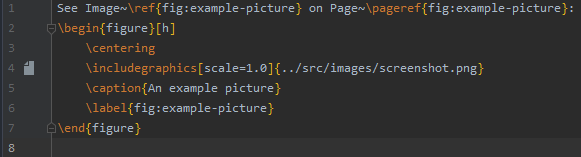
\includegraphics[scale=1.0]{../src/images/screenshot.png}
    \caption{An example picture}
    \label{fig:example-picture}
\end{figure}

Multiple Figures in one environment:
Use hfill for margin between for multi line leave blank lines.
\begin{figure}[hbt!]
    \centering
    \begin{subfigure}[hbt!]{0.49\textwidth}
        \centering
        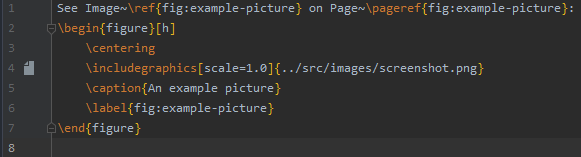
\includegraphics[width=\textwidth]{../src/images/screenshot.png}
        \caption{Picture One}
        \label{fig:one}
    \end{subfigure}
    \hfill
    \begin{subfigure}[hbt!]{0.49\textwidth}
        \centering
        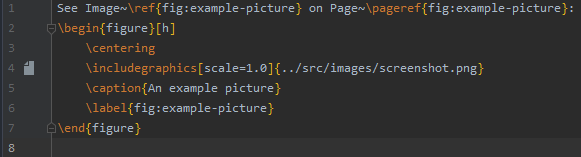
\includegraphics[width=\textwidth]{../src/images/screenshot.png}
        \caption{Picture Two}
        \label{fig:two}
    \end{subfigure}
    \newline
    \begin{subfigure}[hbt!]{\textwidth}
        \centering
        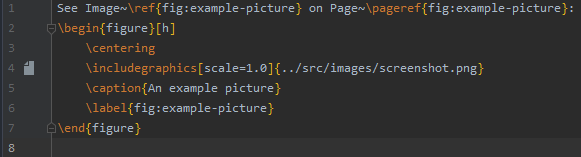
\includegraphics[width=\textwidth]{../src/images/screenshot.png}
        \caption{Picture Three}
        \label{fig:three}
    \end{subfigure}
    \caption{Three pictures}
    \label{fig:three-pictures}
\end{figure}

Reference each fig inside~\ref{fig:three-pictures} like:\newline
One:~\ref{fig:one}\newline
Two:~\ref{fig:two}\newline
Three:~\ref{fig:three}\newline
\clearpage
\section{Tables}\label{sec:tables}
I can reference the table by~\ref{tab:basic-table}
\begin{table}[hbt!]
    \centering
    \begin{tabular}{|l|l|l|}
        A & B & C \\
        \hline
        1 & 2 & 3
    \end{tabular}
    \caption{A basic table}
    \label{tab:basic-table}
\end{table}
See for subtables use:
\begin{table}[hbt!]
    \begin{subtable}[hbt!]{0.45\textwidth}
        \centering
        \begin{tabular}{|l|l|l|}
            A & B & C \\
            \hline
            1 & 2 & 3
        \end{tabular}
        \caption{Multi table 0}
        \label{tab:multi-table-0}
    \end{subtable}
    \hfill
    \begin{subtable}[hbt!]{0.45\textwidth}
        \centering
        \begin{tabular}{|l|l|l|}
            A & B & C \\
            \hline
            1 & 2 & 3
        \end{tabular}
        \caption{Multi table 1}
        \label{tab:multi-table-1}
    \end{subtable}
    \caption{Two tables in one line}
    \label{tab:multi-table}
\end{table}

\section{Minted Code Fragments}\label{sec:minted-code-fragments}

\begin{longlisting}
    \begin{minted}{java}
        public class WaterKettleSteps implements cucumber.api.java8.En {
            @Inject
            public WaterKettleSteps(WaterPage page) {
                When("I waited for \"{int}\" minutes my water is boiling",
                (Integer min) -> {
                    page.assertWaterBoilingAfter(min);
                });
            }
        }

        public class WaterPage {
            public void assertWaterBoilingAfter(Integer min) {
                if (min < 5) { fail(); }
            }
        }
    \end{minted}
    \caption[Short Code Example]{A shorter code example, which will not break across pages.}
    \label{lst:short}
\end{longlisting}

\section{Citation}\label{sec:citation}

Use citation of entry with key rose\textunderscore cucumber\textunderscore 2015: \newline
Citation without brackets with cite\textbraceleft rose\textunderscore cucumber\textunderscore 2015\textbraceright\space like~\cite{rose_cucumber_2015}. \newline
Citation with brackets with parencite\textbraceleft rose\textunderscore cucumber\textunderscore 2015\textbraceright\space like~\parencite{rose_cucumber_2015}.

\chapter{Ipsum chapter}\label{ch:ipsum-chapter}
Lorem ipsum dolor sit amet, consetetur sadipscing elitr, sed diam nonumy eirmod tempor invidunt ut labore et dolore magna aliquyam erat, sed diam voluptua. At vero eos et accusam et justo duo dolores et ea rebum. Stet clita kasd gubergren, no sea takimata sanctus est Lorem ipsum dolor sit amet. Lorem ipsum dolor sit amet, consetetur sadipscing elitr, sed diam nonumy eirmod tempor invidunt ut labore et dolore magna aliquyam erat, sed diam voluptua. At vero eos et accusam et justo duo dolores et ea rebum. Stet clita kasd gubergren, no sea takimata sanctus est Lorem ipsum dolor sit amet. Lorem ipsum dolor sit amet, consetetur sadipscing elitr, sed diam nonumy eirmod tempor invidunt ut labore et dolore magna aliquyam erat, sed diam voluptua. At vero eos et accusam et justo duo dolores et ea rebum. Stet clita kasd gubergren, no sea takimata sanctus est Lorem ipsum dolor sit amet.

Duis autem vel eum iriure dolor in hendrerit in vulputate velit esse molestie consequat, vel illum dolore eu feugiat nulla facilisis at vero eros et accumsan et iusto odio dignissim qui blandit praesent luptatum zzril delenit augue duis dolore te feugait nulla facilisi. Lorem ipsum dolor sit amet, consectetuer adipiscing elit, sed diam nonummy nibh euismod tincidunt ut laoreet dolore magna aliquam erat volutpat.

Ut wisi enim ad minim veniam, quis nostrud exerci tation ullamcorper suscipit lobortis nisl ut aliquip ex ea commodo consequat. Duis autem vel eum iriure dolor in hendrerit in vulputate velit esse molestie consequat, vel illum dolore eu feugiat nulla facilisis at vero eros et accumsan et iusto odio dignissim qui blandit praesent luptatum zzril delenit augue duis dolore te feugait nulla facilisi.

Nam liber tempor cum soluta nobis eleifend option congue nihil imperdiet doming id quod mazim placerat facer possim assum. Lorem ipsum dolor sit amet, consectetuer adipiscing elit, sed diam nonummy nibh euismod tincidunt ut laoreet dolore magna aliquam erat volutpat. Ut wisi enim ad minim veniam, quis nostrud exerci tation ullamcorper suscipit lobortis nisl ut aliquip ex ea commodo consequat.

Duis autem vel eum iriure dolor in hendrerit in vulputate velit esse molestie consequat, vel illum dolore eu feugiat nulla facilisis.

At vero eos et accusam et justo duo dolores et ea rebum. Stet clita kasd gubergren, no sea takimata sanctus est Lorem ipsum dolor sit amet. Lorem ipsum dolor sit amet, consetetur sadipscing elitr, sed diam nonumy eirmod tempor invidunt ut labore et dolore magna aliquyam erat, sed diam voluptua. At vero eos et accusam et justo duo dolores et ea rebum. Stet clita kasd gubergren, no sea takimata sanctus est Lorem ipsum dolor sit amet. Lorem ipsum dolor sit amet, consetetur sadipscing elitr, At accusam aliquyam diam diam dolore dolores duo eirmod eos erat, et nonumy sed tempor et et invidunt justo labore Stet clita ea et gubergren, kasd magna no rebum. sanctus sea sed takimata ut vero voluptua. est Lorem ipsum dolor sit amet. Lorem ipsum dolor sit amet, consetetur sadipscing elitr, sed diam nonumy eirmod tempor invidunt ut labore et dolore magna aliquyam erat.

Consetetur sadipscing elitr, sed diam nonumy eirmod tempor invidunt ut labore et dolore magna aliquyam erat, sed diam voluptua. At vero eos et accusam et justo duo dolores et ea rebum. Stet clita kasd gubergren, no sea takimata sanctus est Lorem ipsum dolor sit amet. Lorem ipsum dolor sit amet, consetetur sadipscing elitr, sed diam nonumy eirmod tempor invidunt ut labore et dolore magna aliquyam erat, sed diam voluptua. At vero eos et accusam et justo duo dolores et ea rebum. Stet clita kasd gubergren, no sea takimata sanctus est Lorem ipsum dolor sit amet. Lorem ipsum dolor sit amet, consetetur sadipscing elitr, sed diam nonumy eirmod tempor invidunt ut labore et dolore magna aliquyam erat, sed diam voluptua. At vero eos et accusam et justo duo dolores et ea rebum. Stet clita kasd gubergren, no sea takimata sanctus.

Lorem ipsum dolor sit amet, consetetur sadipscing elitr, sed diam nonumy eirmod tempor invidunt ut labore et dolore magna aliquyam erat, sed diam voluptua. At vero eos et accusam et justo duo dolores et ea rebum. Stet clita kasd gubergren, no sea takimata sanctus est Lorem ipsum dolor sit amet. Lorem ipsum dolor sit amet, consetetur sadipscing elitr, sed diam nonumy eirmod tempor invidunt ut labore et dolore magna aliquyam erat, sed diam voluptua. At vero eos et accusam et justo duo dolores et ea rebum. Stet clita kasd gubergren, no sea takimata sanctus est Lorem ipsum dolor sit amet. Lorem ipsum dolor sit amet, consetetur sadipscing elitr, sed diam nonumy eirmod tempor invidunt ut labore et dolore magna aliquyam erat, sed diam voluptua. At vero eos et accusam et justo duo dolores et ea rebum. Stet clita kasd gubergren, no sea takimata sanctus est Lorem ipsum dolor sit amet.

Duis autem vel eum iriure dolor in hendrerit in vulputate velit esse molestie consequat, vel illum dolore eu feugiat nulla facilisis at vero eros et accumsan et iusto odio dignissim qui blandit praesent luptatum zzril delenit augue duis dolore te feugait nulla facilisi. Lorem ipsum dolor sit amet, consectetuer adipiscing elit, sed diam nonummy nibh euismod tincidunt ut laoreet dolore magna aliquam erat volutpat.

Ut wisi enim ad minim veniam, quis nostrud exerci tation ullamcorper suscipit lobortis nisl ut aliquip ex ea commodo consequat. Duis autem vel eum iriure dolor in hendrerit in vulputate velit esse molestie consequat, vel illum dolore eu feugiat nulla facilisis at vero eros et accumsan et iusto odio dignissim qui blandit praesent luptatum zzril delenit augue duis dolore te feugait nulla facilisi.

Nam liber tempor cum soluta nobis eleifend option congue nihil imperdiet doming id quod mazim placerat facer possim assum. Lorem ipsum dolor sit amet, consectetuer adipiscing elit, sed diam nonummy nibh euismod tincidunt ut laoreet dolore magna aliquam erat volutpat. Ut wisi enim ad minim veniam, quis nostrud exerci tation ullamcorper suscipit lobortis nisl ut aliquip ex ea commodo



\cleardoublepage
\renewcommand{\thechapter}{\Roman{chapter}}
\setcounter{chapter}{3}
%\pagenumbering{Roman}
\appendix
\addcontentsline{toc}{chapter}{\protect\numberline{V}Appendix}
\chapter*{Appendix}
%Bibliography
\setcounter{biburllcpenalty}{7000} %Adds breakpoints in URLs - https://tex.stackexchange.com/questions/134191/line-breaks-of-long-urls-in-biblatex-bibliography
\setcounter{biburlucpenalty}{8000}
\addcontentsline{toc}{chapter}{\protect\numberline{VI}Bibliography}
\printbibliography

%Eigenständigkeitserklärung
%\input{documents/content/resources/other-pages/6_eidesstatlicheerklaerung.tex}

\end{document}
